\section{方法}
\label{sec:method}
\begin{figure}[tb]
  \centering
  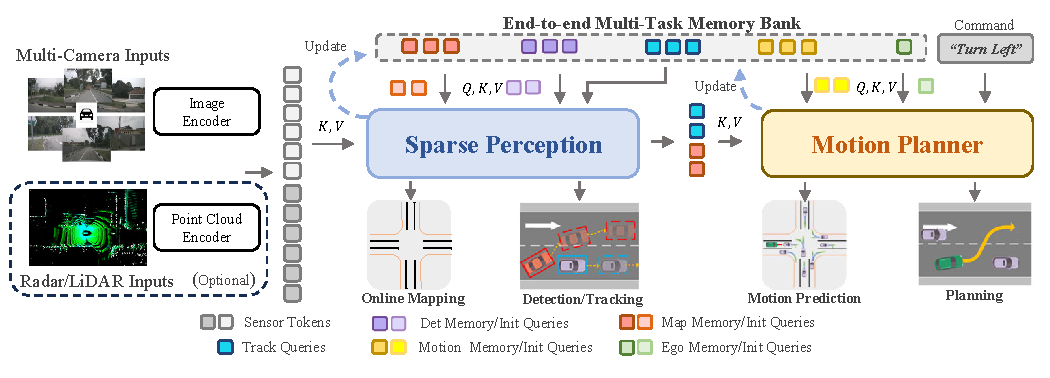
\includegraphics[width=1\linewidth]{Figures/Arch-Figure}
  \caption{\textbf{\model} 的流程，其中稀疏查询完全代表跨空间、时间和任务的驾驶场景，无需任何密集BEV特征。}
  \label{fig:arch}
\end{figure}
\subsection{概述}

如 \cref{fig:pipeline-c} 所示，在所提出的稀疏查询中心（Sparse Query-Centric）范式中，不同的稀疏查询完全代表整个驾驶场景，不仅负责跨模块的信息传递和交互，还在端到端方式下为多任务优化反向传播梯度。与先前密集BEV中心方法 \cite{hu2023planning, jiang2023vad, ye2023fusionad} 不同，本文方法无需任何视图投影器 \cite{philion2020lift} 和密集BEV特征，从而避免了沉重的计算和内存负担 \cite{liu2022petr, jiang2023far3d, zhang2023fully}。

\model 的详细架构如 \cref{fig:arch} 所示。从结构上看，\model 包含三个部分：传感器编码器、稀疏感知和运动规划器。具体而言，传感器编码器将多视角相机图像、雷达或激光雷达点云作为输入，编码为高维特征，这些特征作为传感器令牌（Sensor Token）并附带位置嵌入（PE, Positional Embedding）\cite{liu2022petr, yan2023cross} 输入到稀疏感知模块。在稀疏感知模块中，来自传感器的原始数据将被聚合成多种稀疏感知查询，如检测查询、跟踪查询和地图查询，它们分别表示驾驶场景的不同元素，并将进一步传播到下游任务。在运动规划器中，感知查询被视为驾驶场景的稀疏表示，并针对所有周围智能体和自车进行充分挖掘，然后考虑多个方面的驾驶约束以生成满足安全和运动学要求的最终规划。此外，架构中引入了端到端多任务记忆库（EMMB），用于统一存储整个驾驶场景的时序信息，使全栈驾驶任务能够受益于长时间历史聚合。所提方法的定义和实现细节详见 \cref{appendix-imple}。

\subsection{稀疏感知}
\label{sec:sparse_perception}
\begin{figure}[tb]
  \centering
  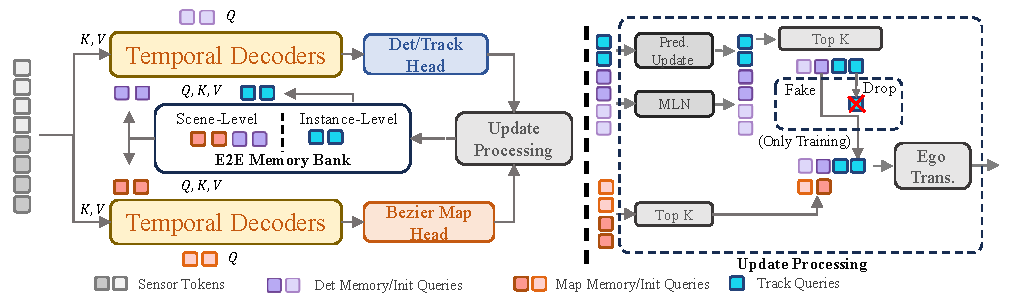
\includegraphics[width=1\linewidth]{Figures/Det-Map-Arch-Figure}
  \caption{\textbf{稀疏感知}模块，由两个统一解码器和两个对应的头部分别用于检测\&跟踪和在线建图。}
  \label{fig:dt-map-arch}
\end{figure}

如 \cref{fig:dt-map-arch} 所示，\model 的稀疏感知模块以稀疏方式统一了包括检测、跟踪和在线建图在内的多感知任务。具体而言，本文采用两个共享完全相同结构的时序解码器 \cite{wang2023exploring}，利用记忆库中的长期历史信息，一个用于障碍物感知，另一个用于在线建图。经过通过不同感知查询进行信息聚合后，应用检测\&跟踪头和贝塞尔地图头分别解码并输出障碍物和地图元素。之后，执行过滤并保存当前帧高置信度感知查询的更新过程，并相应更新记忆库，这将有利于下一帧的感知过程。

\paragraph{\textbf{检测\&跟踪。}} 对于障碍物感知，本文在统一解码器内采用联合检测与跟踪，无需额外的手工后处理。如 \cite{zhang2023motrv2, yu2023motrv3} 研究所指出的，检测查询和跟踪查询之间存在明显的不平衡，可能导致检测性能不可忽视的下降。

为缓解上述问题，本文从多个角度改进障碍物感知性能。首先，引入两层级记忆机制在帧间传播时序信息，其中场景级记忆维护来自查询的信息而无需跨帧关联，实例级记忆保持被跟踪障碍物相邻帧之间的对应关系。其次，考虑到场景级和实例级记忆的来源和任务差异，对两者应用不同的更新策略。具体而言，通过MLN \cite{wang2023exploring} 更新场景级记忆，而实例级记忆通过每个障碍物的未来预测进行更新。此外，在训练中对跟踪查询采用增强策略 \cite{zeng2022motr} 以平衡两层级记忆之间的监督，从而提升检测和跟踪性能。

随后，通过检测\&跟踪头从检测或跟踪查询中解码出带有属性和唯一ID的3D边界框，并进一步用于下游任务。

\paragraph{\textbf{在线建图。}} 据本文所知，现有的在线建图方法均依赖密集BEV特征表示驾驶环境，这使得由于高内存和计算成本而难以扩大感知范围或利用历史信息。基于所有地图元素都可以用稀疏方式表示的认知和信念，本文尝试在稀疏范式中实现在线建图。

具体而言，本文采用与障碍物感知任务中结构相同的时序解码器。初始时，带有先验类别的地图查询被初始化并均匀分布在驾驶平面上。在时序解码器中，地图查询与传感器令牌和历史记忆令牌（实际上由先前帧中高置信度的地图查询组成）进行交互。然后，携带当前帧地图元素有效信息的更新后地图查询可被推入记忆库，以便在后续帧或下游任务中使用。显然，在线建图的流程与障碍物感知基本相同。也就是说，本文以通用的稀疏方式统一了包括检测、跟踪和在线建图在内的感知任务，这种方式能够更高效地扩展到更大范围（如 $100m\times100m$）或长期时序融合，无需复杂的算子（如可变形注意力\cite{zhu2020deformable}、多点注意力\cite{yuan2024streammapnet}）。据本文所知，本文首次在统一的稀疏感知架构中以稀疏方式实现在线建图。

随后，利用分段贝塞尔（Bezier）\cite{qiao2023end} 地图头回归每个稀疏地图元素的分段贝塞尔控制点，这些控制点可方便地转换为下游任务所需的形式。

\subsection{运动规划器}
\label{sec:motion_planner}

本文重新审视了自动驾驶系统中的运动预测和规划，并认识到许多先前方法 \cite{shi2024mtr++, zhou2022hivt} 在对周围智能体进行运动预测时忽略了自车。虽然在大多数情况下该问题并不显现，但在近处智能体与自车存在强交互的场景（如交叉路口）中可能存在潜在风险。
基于上述认识，本文设计了一个更合理的运动规划器框架，其中运动预测器同时对周围智能体和自车进行运动预测。自车的预测结果随后作为运动先验用于后续的规划优化器。
然后综合考虑不同方面的约束以生成同时满足安全和运动学要求的最终规划结果。

\begin{figure}[tb]
  \centering
  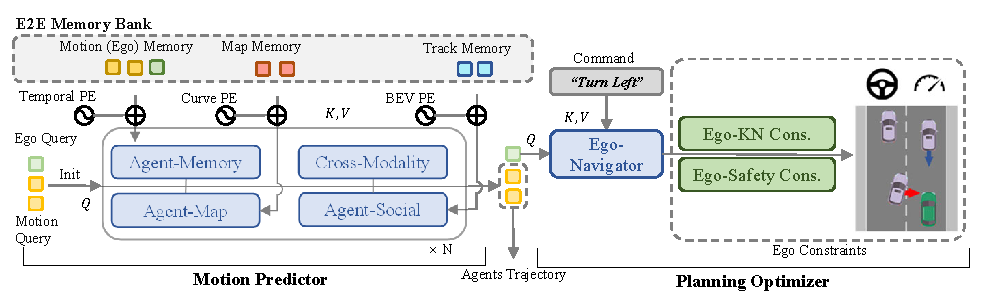
\includegraphics[width=1\linewidth]{Figures/MotionPlanner-Arch-Figure}
  \caption{\textbf{运动规划器}模块考虑不同智能体与自车之间的关系，以及安全和运动学方面的驾驶约束。}
  \label{fig:fore-arch}
\end{figure}

如 \cref{fig:fore-arch} 所示，\model 中的运动规划器将包含跟踪查询和地图查询的感知查询作为当前驾驶场景的稀疏表示，多模态运动查询（Motion Query）作为实现驾驶场景感知、所有智能体（包括自车）之间交互以及不同未来可能性之间博弈的媒介。然后自车的多模态运动查询被送入规划优化器，其中多个方面的驾驶约束（包括高级指令、安全和运动学）以不同方式得到充分考虑。

\paragraph{\textbf{运动预测器。}} 遵循先前方法 \cite{hu2023planning, ye2023fusionad}，运动查询与当前驾驶场景表示（包括跟踪查询和地图查询）之间的感知和交互通过标准Transformer \cite{vaswani2017attention} 层实现。此外，应用自车-智能体和跨模态交互，在未来的时空场景中联合建模周围智能体和自车之间的交互。借助上述多层堆叠结构内部及之间的协同作用，运动查询能够从静态和动态环境中聚合丰富的语义信息。

除上述内容外，本文还引入了两种策略进一步提升运动预测器的性能。首先，使用跟踪查询的实例级时序记忆进行简单直接的预测，并将其作为周围智能体运动查询的部分初始化。通过这种方式，运动预测器能够受益于上游任务获得的先验信息。其次，得益于端到端记忆库，通过智能体-记忆聚合器以几乎可忽略的成本以流式方式吸收保存的历史运动查询中的有用信息。

需要指出的是，自车的多模态运动查询同时得到更新。通过这种方式能够获得自车的运动先验，从而进一步促进规划的学习过程。

\paragraph{\textbf{规划优化器。}} 借助运动预测器提供的运动先验，获得更好的初始化，在训练过程中减少走弯路。作为运动规划器的关键组件，代价函数的设计至关重要，因为它将极大影响甚至决定最终的性能。在\model 的运动规划器中，从安全和运动学两个主要方面考虑不同的约束，旨在生成令人满意的规划结果。

具体而言，除了VAD\cite{jiang2023vad} 中定义的约束外，本文特别关注自车与附近智能体之间的动态安全关系，考虑它们在未来的相对位置。例如，如果智能体 $i$ 持续保持在自车的前方左侧区域，从而阻止自车向左行驶，则该智能体 $i$ 将获得\textit{left}标签，表示智能体 $i$ 对自车施加了左侧约束（详见 \cref{appendix-imple-motionplanner}）。相应地，在纵向方向上将约束分类为\textit{front}、\textit{back}或\textit{no}，在横向方向上将约束分类为\textit{left}、\textit{right}或\textit{no}。
在运动规划器中，从对应查询中解码出其他智能体与自车在横向和纵向方向上的关系。该过程涉及确定所有其他智能体与自车在这些方向上的约束关系概率。
然后利用焦点损失（Focal Loss）\cite{lin2017focal} 作为自车-智能体关系（EAR, Ego-Agent Relationship）的代价函数，有效捕捉来自附近智能体的潜在风险：

\begin{equation}
    \mathcal{L}_{EAR} = - \sum_{d=1}^D\sum_{i=1}^A\sum_{c=1}^C\alpha_i(1-\hat{R^d_{ic}})^\gamma \log(\hat{R^d_{ic}})
\end{equation}
其中 $A$ 表示周围智能体数量，$C$ 表示类别数量，$D$ 为约束方向数量（纵向和横向），$\alpha_i$ 和 $\gamma$ 是焦点损失中的超参数。
使用 \(\hat{R}^d_{ic}\) 表示智能体 $i$ 在方向 $d$ 上属于关系 $c$ 的概率。

由于规划轨迹必须符合运动学规律以便控制系统执行，在运动规划器中嵌入了辅助任务以促进自车运动状态的学习。从自车查询 $Q_{\text{ego}}$ 中解码出速度、加速度和偏航角等状态，并通过运动学损失进行监督：

\begin{equation}
    L_{\text{KN}} = \frac{1}{N} \sum_{i=1}^{N} \left(\textrm{Dec}(Q_{\text{ego}})_i - \text{status}_i\right)^2
\end{equation}
其中 $N$ 表示自车状态的数量，$\text{status}_i$ 表示自车的第 $i$ 个实际状态。
